\documentclass[UTF8]{article}
\usepackage{ctex}
% if you need to pass options to natbib, use, e.g.:
%\PassOptionsToPackage{numbers, compress}{natbib}
% before loading neurips_2022

\usepackage{setspace}
\singlespacing
% ready for submission
%\usepackage{neurips_2022}

% to compile a preprint version, e.g., for submission to arXiv, add add the
% [preprint] option:
\usepackage[preprint]{neurips_2022}

% to compile a camera-ready version, add the [final] option, e.g.:
%\usepackage[final]{neurips_2022}


% to avoid loading the natbib package, add option nonatbib:
%\usepackage[nonatbib]{neurips_2022}

\usepackage[utf8]{inputenc} % allow utf-8 input
\usepackage[T1]{fontenc}    % use 8-bit T1 fonts
\usepackage{hyperref}       % hyperlinks
\usepackage{url}            % simple URL typesetting          
\usepackage{booktabs}       % professional-quality tables
\usepackage{amsfonts}       % blackboard math symbols
\usepackage{nicefrac}       % compact symbols for 1/2, etc.
\usepackage{microtype}      % microtypography
\usepackage{xcolor}         % colors
\usepackage{amsmath}
\usepackage{graphicx}
\usepackage{float}
\usepackage{subfig}
\usepackage[ruled,vlined]{algorithm2e}
\usepackage{xcolor}

\captionsetup[figure]{name=Figure}
\renewcommand{\refname}{References}

\title{Penetrating the "Grokking" Phenomenon}


% The \author macro works with any number of authors. There are two commands
% used to separate the names and addresses of multiple authors: \And and \AND.
%
% Using \And between authors leaves it to LaTeX to determine where to break the
% lines. Using \AND forces a line break at that point. So, if LaTeX puts 3 of 4
% authors names on the first line, and the last on the second line, try using
% \AND instead of \And before the third author name.


\author{
  陈风凌 \\
  School of Mathematical Sciences\\
  Student id: \texttt{2200010890}
  % examples of more authors
  \And
  贾沛文 \\
  Guanghua School of Management \\
  Student id: \texttt{2201111026}
  \AND
  汪晨阳 \\
  School of Mathematical Sciences\\
  Student id: \texttt{2200010865}
}


\begin{document}


\maketitle


\begin{abstract}
  This article is concerned about the Grokking phenomenon in the learning of modular addition. Starting from transformer models with AdamW optimizer, we perform experiments investigate the effect of training fraction on the training and validation accuracy. Other model structures, optimizers and regularization techniques are considered. We also explore Grokking in multivariate modular addition. Lastly, we adopt the Grokfast algorithm and provide a possible explanation of Grokking. 
  The code of our experiments can be accessed at
  \href{https://github.com/jpw2022/Introduction-to-ML}{our github repository}.
\end{abstract}

\paragraph{Keywords} Grokking; modular addition; Grokfast; transformer; Adam

\section{Introduction}
In machine learning, the ``Grokking'' phenomenon refers to a sudden, unexpected breakthrough in the model's learning process, typically occurring when the model reaches a very low training error. It often appears as a sudden, dramatic improvement in performance after a period of seemingly slow learning. This phenomenon is particularly surprising because, before grokking, the model might have struggled with overfitting or faced training challenges, and after grokking, it generally performs exceptionally well. In short, grokking is when a model "suddenly gets it" and improves significantly, often exceeding expectations, see, for example, \cite{power2022grokking}, \cite{lee2024grokfast}, \cite{mohamadi2024you}, \cite{kumar2023grokking} and 
\cite{lyu2023dichotomy}. 

In this paper, we aim to investigate the Grokking phenomenon in the learning of modular addition. We will replicate some results in \cite{power2022grokking} via various models, optimizers and regularization techniques. After that, some discussion on Grokking is provided. 
 

\section{The problem and data}
Formally, we want to explore the learning of (binary) modular addition
\begin{equation*}
(x,y) \mapsto x+y~ \mathrm{mod} ~ p, \quad \text{for}~ x,y \in \mathbb{Z}_p.
\end{equation*}  

Each token ``$x$'', ``$+$'', ``$y$'', ``$=$'' and the outcome ``$x+y~ \mathrm{mod} ~ p$'' is embedded into a one-hot vector with length $p+2$. Here the dimension $p+2$ is due to the additional tokens ``$+$'' and ``$=$'', which are embedded as $(0,\ldots,1,0)_{1\times (p+2)}$ and $(0,\ldots,0,1)_{1\times (p+2)}$ repectively. Here is a toy example of $p=3$. Let $x=1$, $y=2$, then ``$x$'', ``$+$'', ``$y$'', ``$=$'' and ``$x+y~ \mathrm{mod} ~ p $'' (i.e. ``$0$'') are encoded as $(0,1,0,0,0)$, $(0,0,0,1,0)$, $(0,0,1,0,0)$, $(0,0,0,0,1)$ and $(1,0,0,0,0)$, respectively. The size of total data is $p^2$. We choose $p=97$ here and afterwards without loss of generality, while larger $p$ corresponds a harder problem.

\section{Experiments}

\subsection{Grokking for transformer models}\label{section_transformer}

We first study the impact of the fraction of training set $\alpha \in (0,1)$ on
the Grokking phenomenon for transformer models using the AdamW optimizer
with weight decay $0.05$ and learning rate $10^{-3}$.
Specifically, the transformer model used has  2 layers and 4 attention heads.
The embedding dimension is 128, and the batchsize set as 256.
Figure \ref{transformer} plots the relationship the
training/validation accuracy and the number of epochs corresponding to $\alpha
\in \{0.3,0.4,0.5,0.7\}$. The Grokking phenomenon does occur such that both
training and validation accuracy rise quickly after a long while of slow
learning, and the validation accuracy starts to rise after the training one
begins.

The effects of training fraction $\alpha$ can also be found from the
four pictures. On the one hand, larger $\alpha$ leads to faster Grokking. For
instance, when $\alpha=0.3$, it takes more than $10^3$ epochs before the
validation accuracy starts to rise, whereas, in comparison, it only takes about
100 epochs when
$\alpha=0.5$. On the other hand, the gap between the training and validation accuracy is narrowed with the increase of $\alpha$. A notable evidence is that when $\alpha$ reaches 0.7, the two accuracy curves seem to rise simultaneously.

\begin{figure}[htb]
  \vspace{-6mm}
  \centering
  %\includegraphics[width=3in]{fig5}
  \subfloat[Training and validation accuracy\\ with $\alpha=0.3$ ]{
      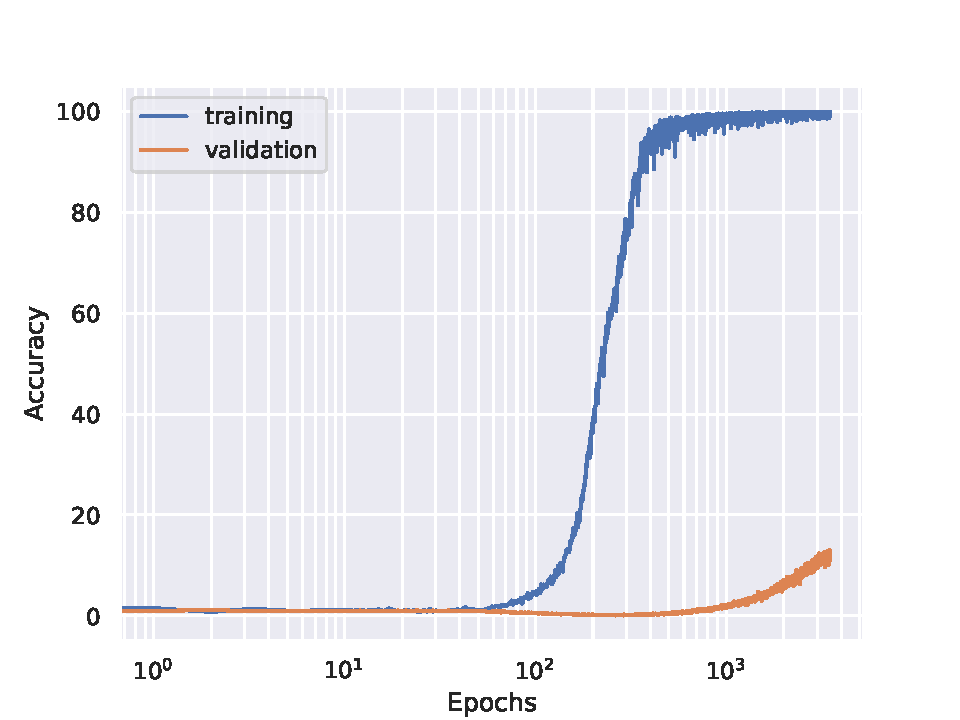
\includegraphics[width=0.5\textwidth]{alpha=0.3.pdf}}
  \subfloat[Training and validation accuracy\\ with $\alpha=0.4$]{
      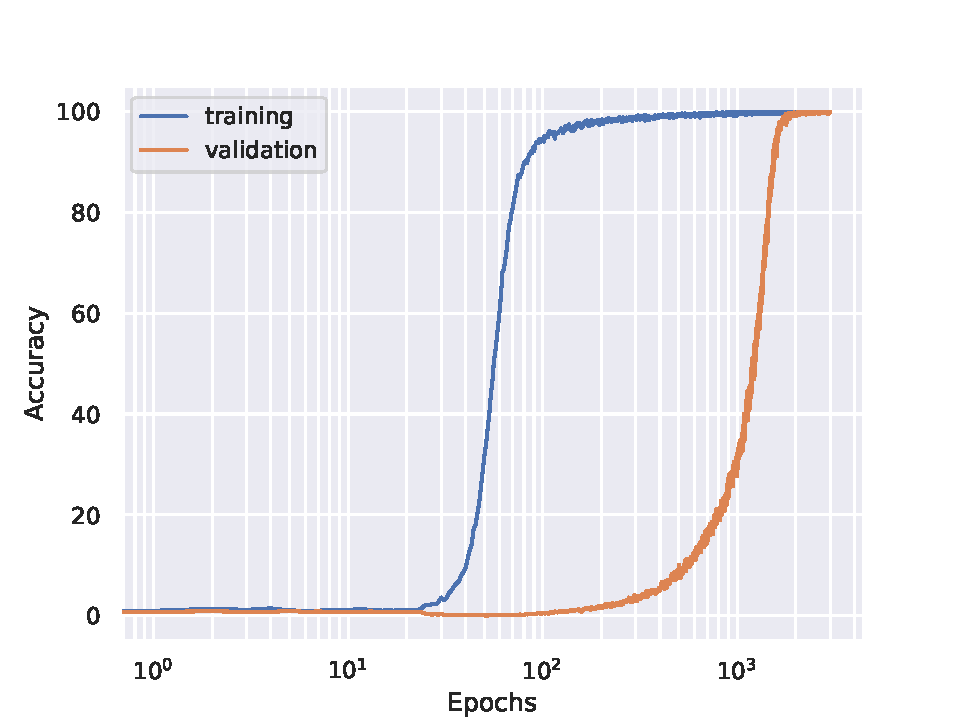
\includegraphics[width=0.5\textwidth]{alpha=0.4.pdf}}
  \\
  \subfloat[Training and validation accuracy\\ with $\alpha=0.5$ \label{transformer_0.5}]{
      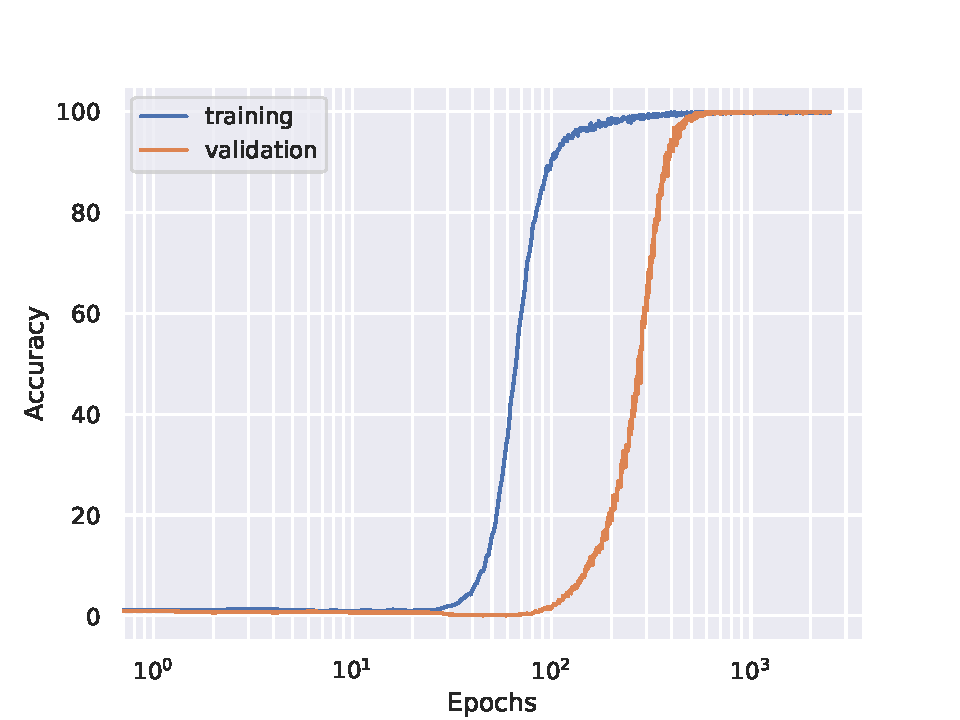
\includegraphics[width=0.5\textwidth]{alpha=0.5.pdf}} 
  \subfloat[Training and validation accuracy\\ with $\alpha=0.7$]{
      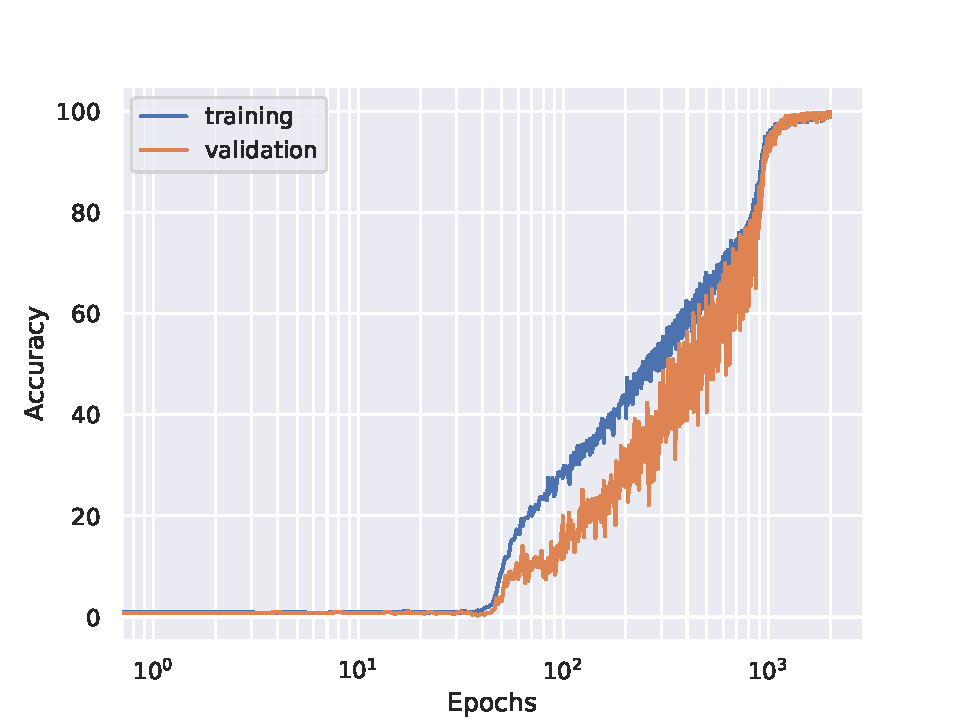
\includegraphics[width=0.5\textwidth]{alpha=0.7.pdf}}
  \caption{Grokking phenomenon on transformer model with different training fraction $\alpha$}
  \label{transformer}
\end{figure}
  

\subsection{Grokking with other network achitectures}

In order to investigate the Grokking on other models, we perform the same experiments with MLP and LSTM. The MLP and LSTM both have two hidden layers of dimension 512. The batchsize dimension and the learning rate mainly follow the settings in Section \ref{section_transformer} for the convenience of comparison. The training and validation accuracy for MLP and LSTM with $\alpha=0.5$ are displayed in Figure \ref{mlplstm}. The Grokking phenomenon also appears in the two models we consider. In contrast to transformer models with the same $\alpha=0.5$ in Figure \ref{transformer_0.5}, it takes fewer epochs before the training accuracy begins to rise, while it is the opposite case for validation accuracy. Moreover, the validation accuracy of these two models increases with significant fluctuations, indicating unstable generalization ability.

\begin{figure}[htb]
  \centering
  \vspace{-6mm}
  %\includegraphics[width=3in]{fig5}
  \subfloat[Training and validation accuracy of MLP\\ with $\alpha=0.5$ ]{
      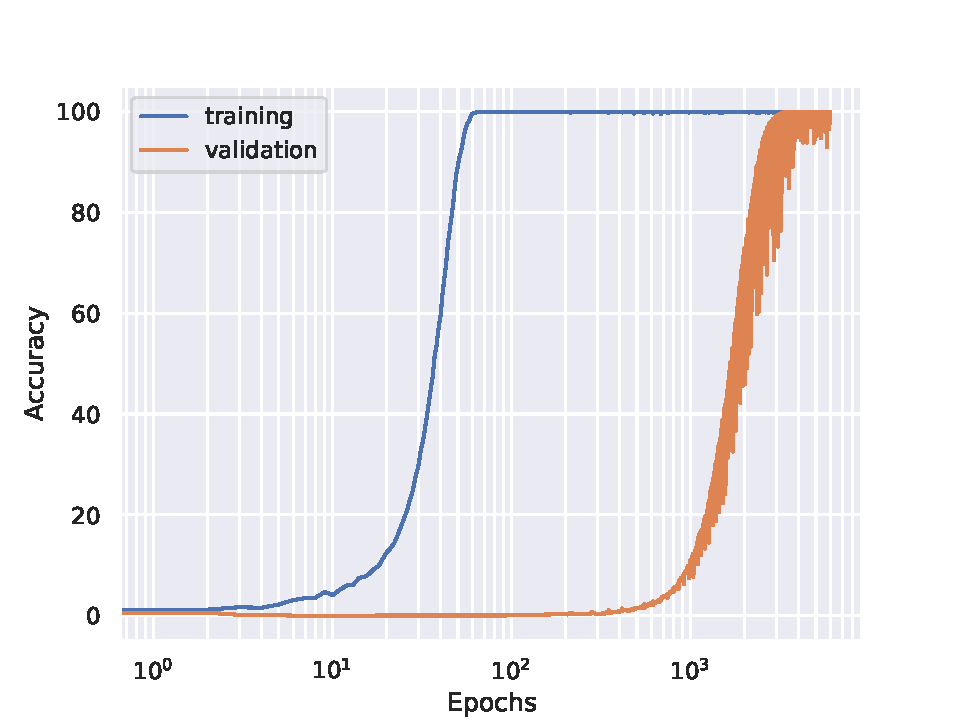
\includegraphics[width=0.5\textwidth]{mlp_0.5.pdf}}
  \subfloat[Training and validation accuracy of LSTM\\ with $\alpha=0.5$]{
      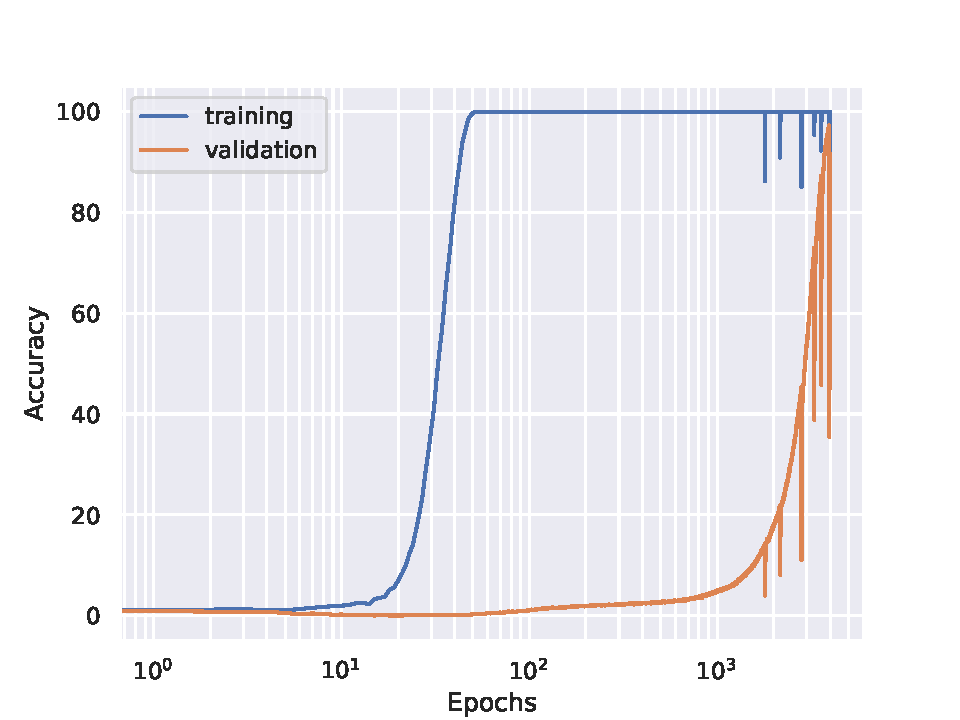
\includegraphics[width=0.5\textwidth]{lstm_0.5.pdf}}
  \caption{Grokking phenomenon on MLP and LSTM with $\alpha=0.5$}
  \label{mlplstm}
\end{figure}

\subsection{The effects of different optimizers and regularization techniques}
In this section, we will focus on the impact of optimizers and regularization
techniques on Grokking for transformer models. For  optimizers, we consider SGD
and SGD with Nesterov momentum (where we set the momentum parameter as
0.9) as competitors against Adam. The maximum validation accuracy with different
training fraction $\alpha$ within an optimization budget of $8000$ steps with
batch size $256$ is plotted in Figure \ref{optimizers}.

It is shown that in
contrast with Adam, the validation accuracy with SGD and SGD nesterov remains at a relatively low level within the optimization budget we consider for each $\alpha$. This is mainly because Adam can quickly adapt and adjust parameters in the early stages of training, it typically converges to a better solution faster than SGD. Besides, Adam has better adaptability to gradient noise and sparse gradients, making the training process more stable.

\begin{figure}[H]
  \centering
  \vspace{-6mm}
  %\includegraphics[width=3in]{fig5}
  \subfloat[Adam]{
      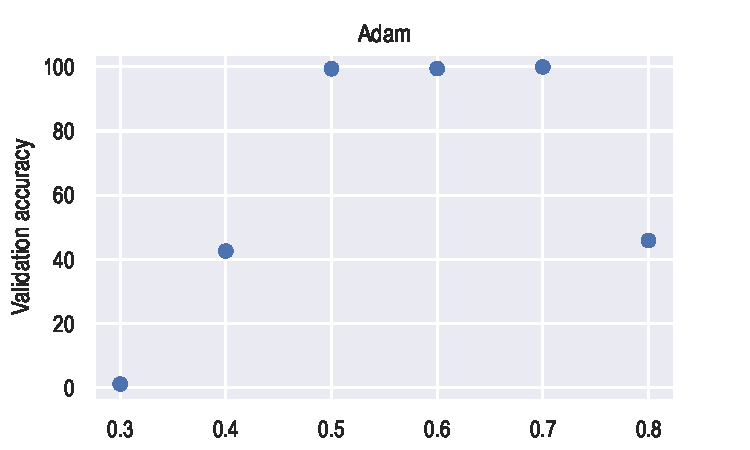
\includegraphics[width=0.35\textwidth ]{Adam_summary.pdf}\label{Adam}}
  \subfloat[SGD]{
      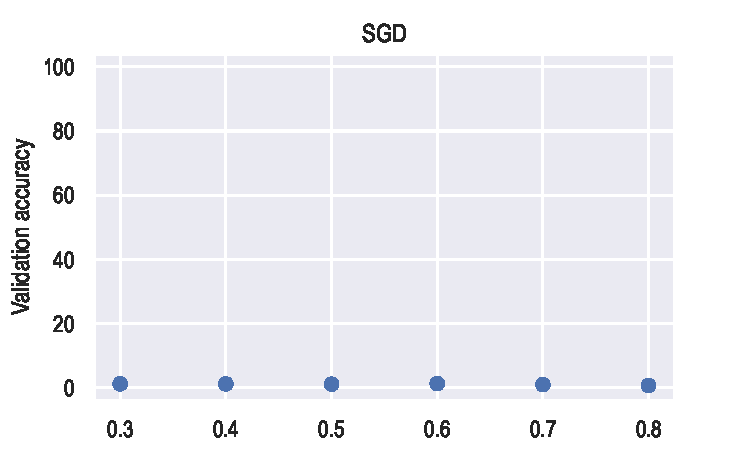
\includegraphics[width=0.35\textwidth ]{SGD_summary.pdf}}
  \subfloat[SGD nesterov]{
      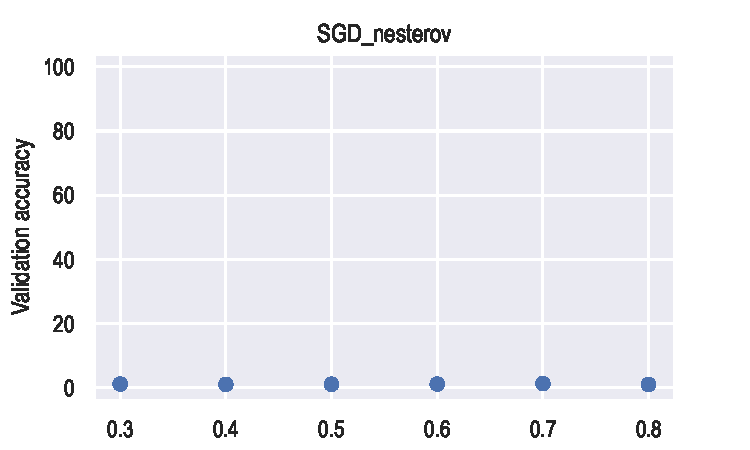
\includegraphics[width=0.35\textwidth ]{SGD_nesterov_summary.pdf}}
  \caption{The maximum
  validation accuracy with different optimizers within an optimization budget of
$8000$ steps}
  \label{optimizers} 
\end{figure}

For the regularization techniques, we consider weight decay of $0.05$ (i.e, AdamW) and dropout (with probability 0.1) for transformer models with Adam optimizer. The corresponding results can be found in Figure \ref{regularization}. Compared with Adam in Figure \ref{Adam}, AdamW (Figure \ref{AdamW}) improves the validation accuracy at $\alpha=0.3$ and $0.8$, while Adam with dropout (Figure \ref{Adamdropout}) performs better at $\alpha=0.8$ but worse at $\alpha=0.5$ and $0.6$.

\begin{figure}[H]
  \centering
  \vspace{-6mm}
  %\includegraphics[width=3in]{fig5}
  \subfloat[AdamW]{
      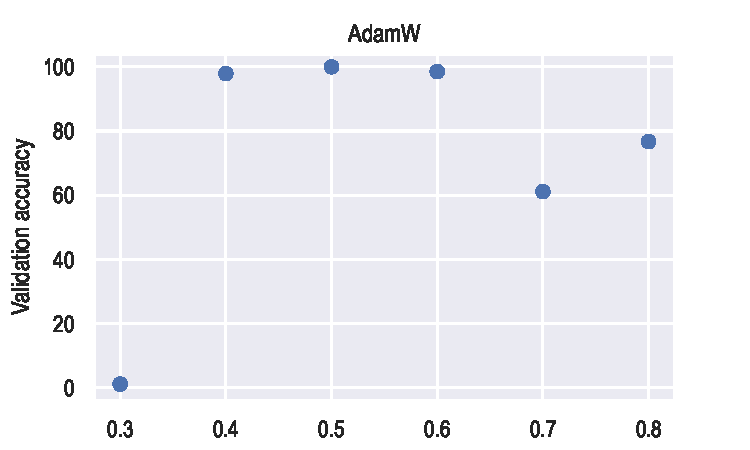
\includegraphics[width=0.35\textwidth ]{AdamW_summary.pdf}\label{AdamW}}
  \subfloat[Adam with dropout]{
      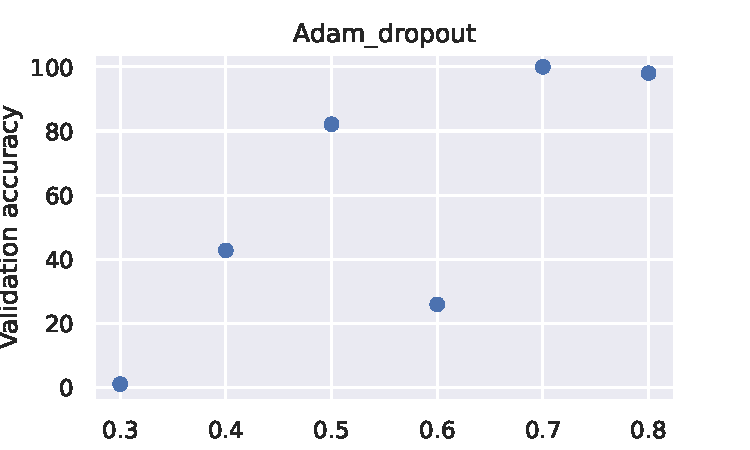
\includegraphics[width=0.35\textwidth ]{Adam_dropout_summary.pdf}\label{Adamdropout}}
  \caption{The maximum
  validation accuracy with different regularization techniques within an
optimization budget of $8000$ steps}
  \label{regularization} 
\end{figure}

In addition, we also conider the Grokfast algorithm introduced by \cite{lee2024grokfast}, which is detailed as Algorithm \ref{algorithm_Grokfast}. Grokfast can simultaneously implement momentum, weight decay, and the filtering. In our experiments, the initial parameters window size $w$ and scalar factor $\lambda$ are set according to the values in \cite{lee2024grokfast}. Figure plots \ref{grokfast} the training and validation accuracy with Grokfast. In fact, Grokfast without filter (Figure \ref{grokfast_nofilter}) is analogous to AdamW, and the filter (Figure \ref{grokfast_filter})
accelerates the generalization.

\begin{algorithm}[H] \label{algorithm_Grokfast}
  \caption{\textsc{Grokfast}}
  \textbf{Param:} window size $w$, scalar factor $\lambda$.\\
  \textbf{Input:} initial parameters $\theta_0$, stochastic objective function $f(\theta)$, optimizer's parameter update $u(g, t)$ from gradient $g$ at timestep $t$.\\
  \textbf{begin:} $t \gets 0$ ; $Q \gets$ Queue(capacity = $w$)\;
  \While{$\theta_t$ not converged}{
      $t \gets t + 1$\;
      $g_t \gets \nabla_\theta f(\theta_{t-1})$ \tcp*[r]{Calculate gradients}
      Insert$(Q, g_t)$ \tcp*[r]{Insert gradients to $Q$}
      $\hat{g}_t \gets g_t + \lambda \cdot \text{Avg}(Q)$ \tcp*[r]{Filter gradients}
      $\hat{u}_t \gets u(\hat{g}_t, t)$ \tcp*[r]{Calculate update}
      $\theta_t \gets \theta_{t-1} + \hat{u}_t$ \tcp*[r]{Update parameters}
  }
  \textbf{end while}.
  \end{algorithm}
  
  \begin{figure}[H]
    \centering
    \vspace{-6mm}
    %\includegraphics[width=3in]{fig5}
    \subfloat[Grokfast with fliter]{
        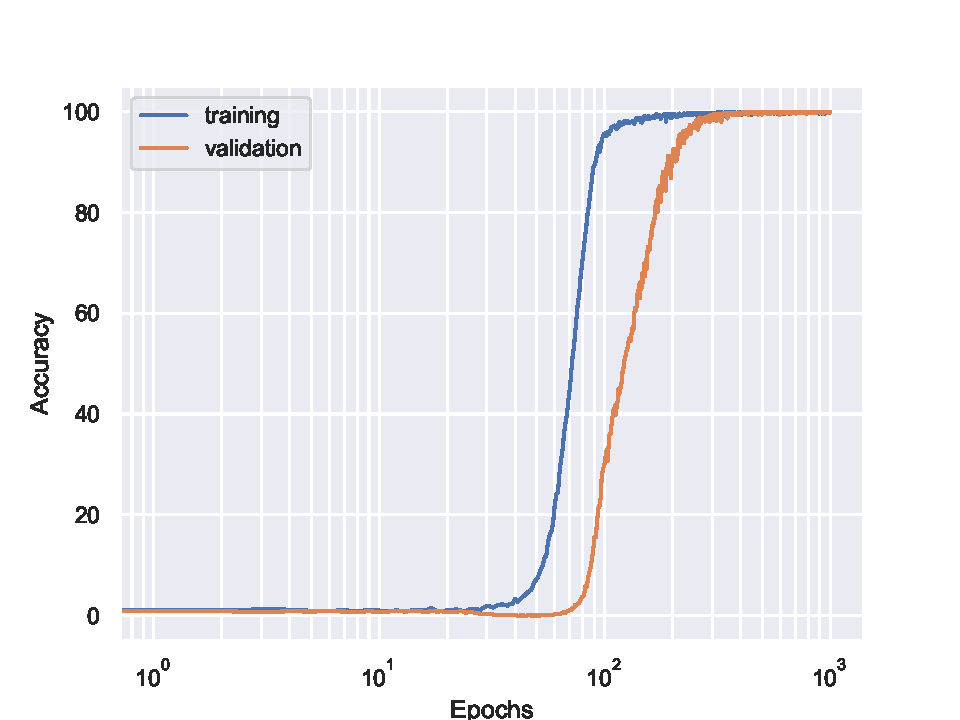
\includegraphics[width=0.5\textwidth]{grokfast with fliter.pdf}\label{grokfast_filter}}
    \subfloat[Grokfast without fliter]{
        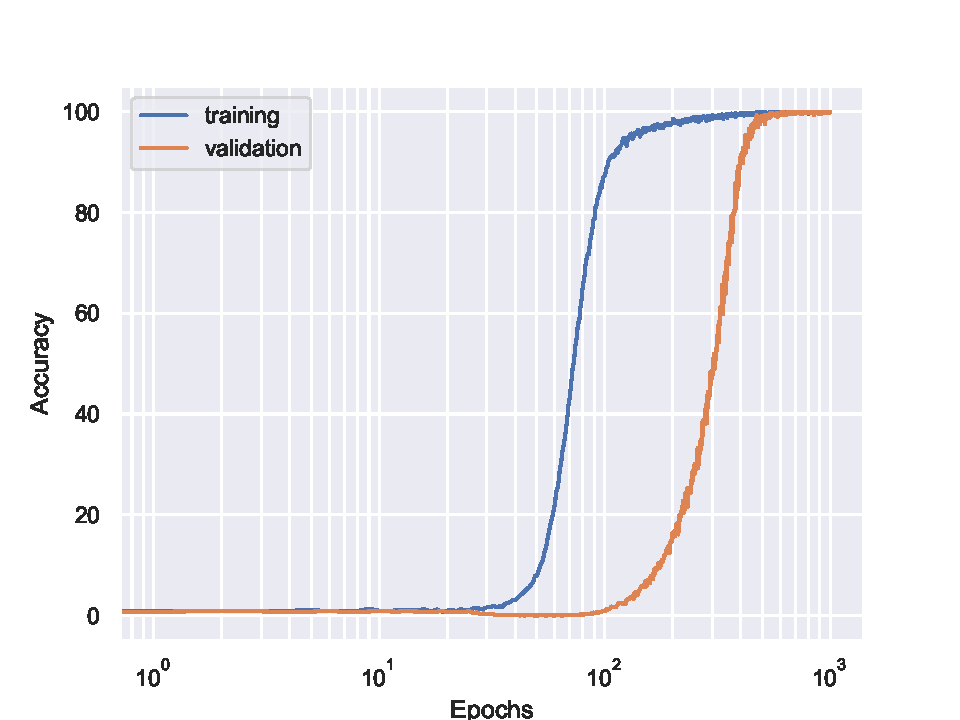
\includegraphics[width=0.5\textwidth]{grokfast without fliter.pdf}\label{grokfast_nofilter}}
    \caption{Training and validation accuracy with Grokfast for $\alpha=0.5$}
    \label{grokfast}
  \end{figure}

\subsection{A harder problem: multivariate modular addition}
In this section we consider the learning of multivariate modular addition as an extention. Specifically, the problem is
\begin{equation*}
  (x_1,\ldots,x_K) \mapsto \left(\sum_{k=1}^K x_k \right)~ \mathrm{mod} ~ p, 
\end{equation*}
where $x_k \in [p]$ for $k=1,\ldots,K$. Our goal is to find the influence of the
dimension $K$ on the Grokking phenomenon. We use the same transformer model as
set in Section \ref{section_transformer}. To start, we first consider the case $K=3$.

Figure \ref{K=3} shows the training and validation accuracy with and without
pretraining. We pretrain the model on $K=2$ data for $2000$ epochs,
and then use a $K=3$ dataset of size $10^4$ to train another $2000$ epochs.
Figures \ref{k3_p97-pre} shows the accuracy of total $4000$ epochs,
while \ref{k3_p97-pre_2} shows the last $2000$ epochs after pretraining.
In order to conduct a fair comparision, for unpretrained model we used
two different $K=3$ dataset of size $10^4$ and train the model on each dataset
for $2000$ epochs.

For unpretrained models, we do not see Grokking for the validation
accuracy within the range of epochs in Figure \ref{k3_nonpre}, while the
training accuracy does grok (the breakpoint is a checkpoint, and so is the
breakpoint in Figure \ref{k3_p97-pre}). On the contrary, for pretrained models,
we can see the Grokking phonomenon within fewer epochs for both training and
validation accuracy, see Figures \ref{k3_p97-pre} and
\ref{k3_p97-pre_2}. Besides, when $K=2$ is
pretrained, the validation accuracy even groks faster than the training
accuracy. Therefore, the pretraining of smaller $K$ will be helpful for the
learning of larger $K$.

\begin{figure}[H]
  \centering
  %\includegraphics[width=3in]{fig5}
  \subfloat[Training and validation accuracy\\ without pretrained ]{
      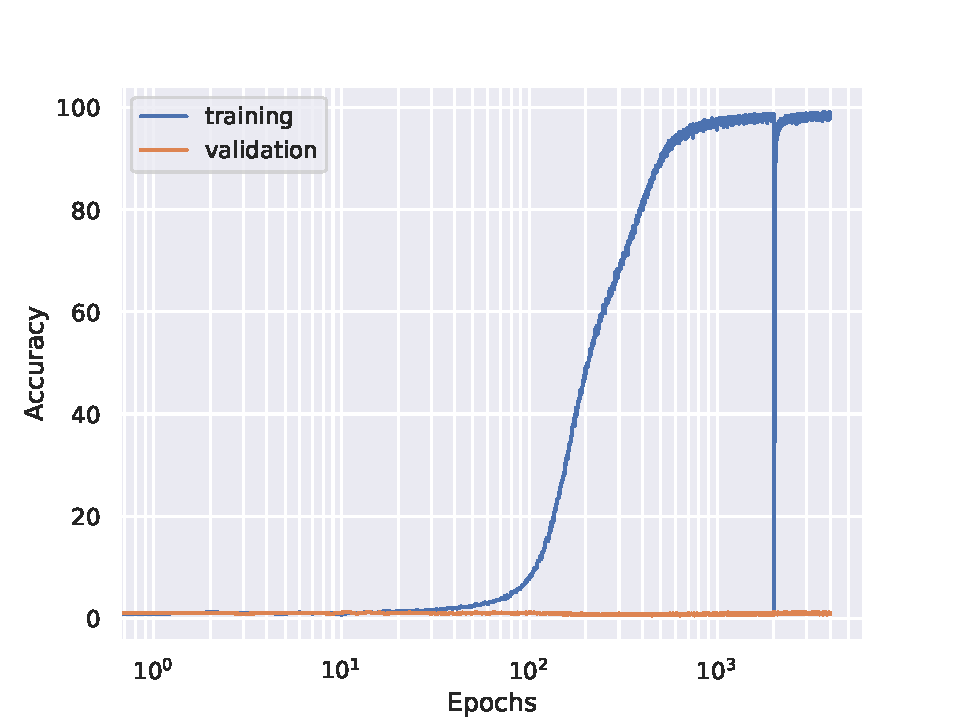
\includegraphics[width=0.35\textwidth]{k3_p97.pdf}\label{k3_nonpre}}
  \subfloat[Training and validation accuracy\\ with $K=2$ pretrained]{
      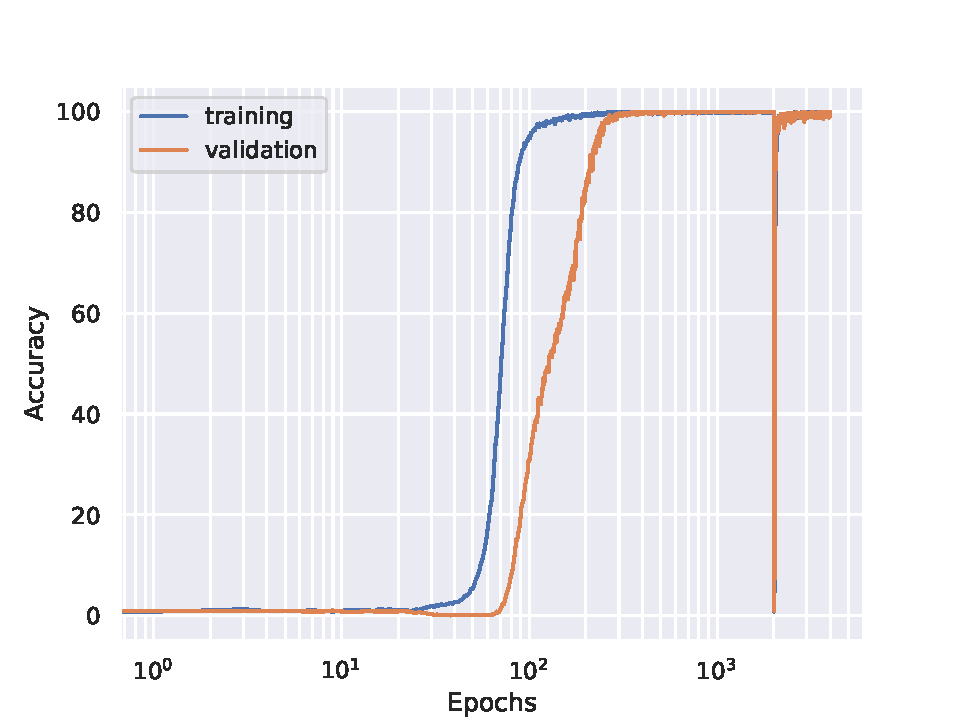
\includegraphics[width=0.35\textwidth]{k3_p97-pre.pdf}\label{k3_p97-pre}}
  \subfloat[Training and validation accuracy\\ after pretraining]{
      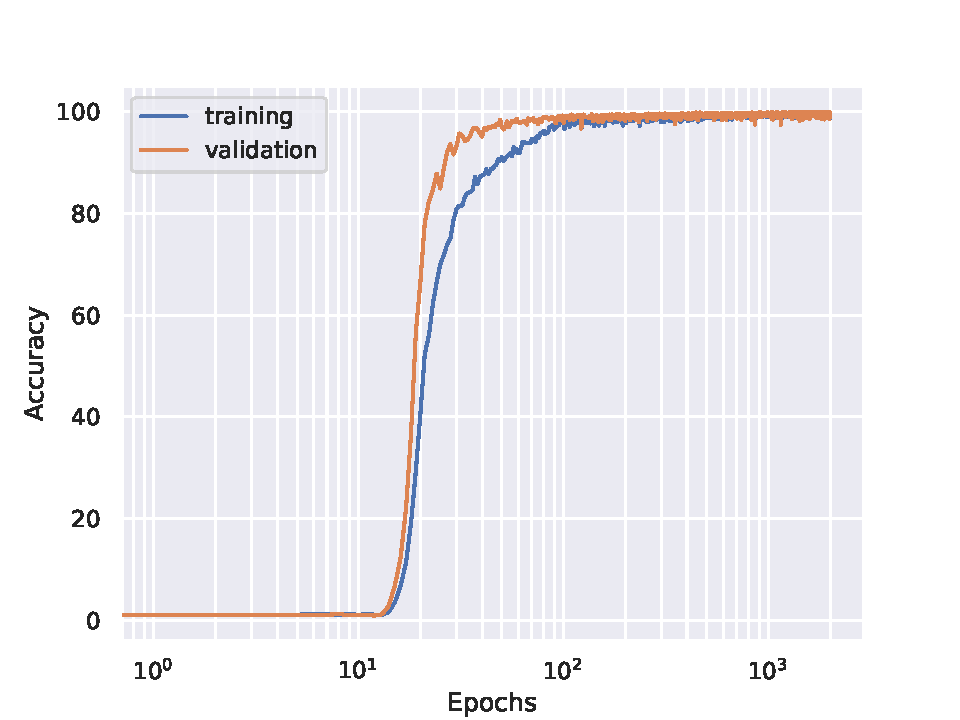
\includegraphics[width=0.35\textwidth]{k3_p97-pre_2.pdf}\label{k3_p97-pre_2}}
  \caption{Grokking phenomenon on transformer model with $K=3$}
  \label{K=3} 
\end{figure}

Based on the above findings, we perform experiments for $K=4,5,6$ with $K=2$ pretrained. The results are displayed in Figure \ref{K=4,5,6}. Compared with Figure \ref{k3_p97-pre_2}, the training accuracy still groks even though a little bit later than $K=3$. However, the validation accuracy shows unstable performance: when $K=4$ (see Figure \ref{k=4}), it rises to about 0.5 and then gradually decreases; when $K=6$ (see Figure \ref{k=6}), it does not grok within the range of epochs plotted. This implies the ``curse of dimension'' such that the larger $K$ corresponds to a harder task to learn and generalize.

We found that when $K=4$, the performance is rather strange. We conjecture
that there are some similar structures of $K=2$ and $K=4$, the model learns
this structure at first instead of correct modular addition.

\begin{figure}[H]
  \centering
  %\includegraphics[width=3in]{fig5}
  \subfloat[Training and validation accuracy\\ with $K=4$ ]{
      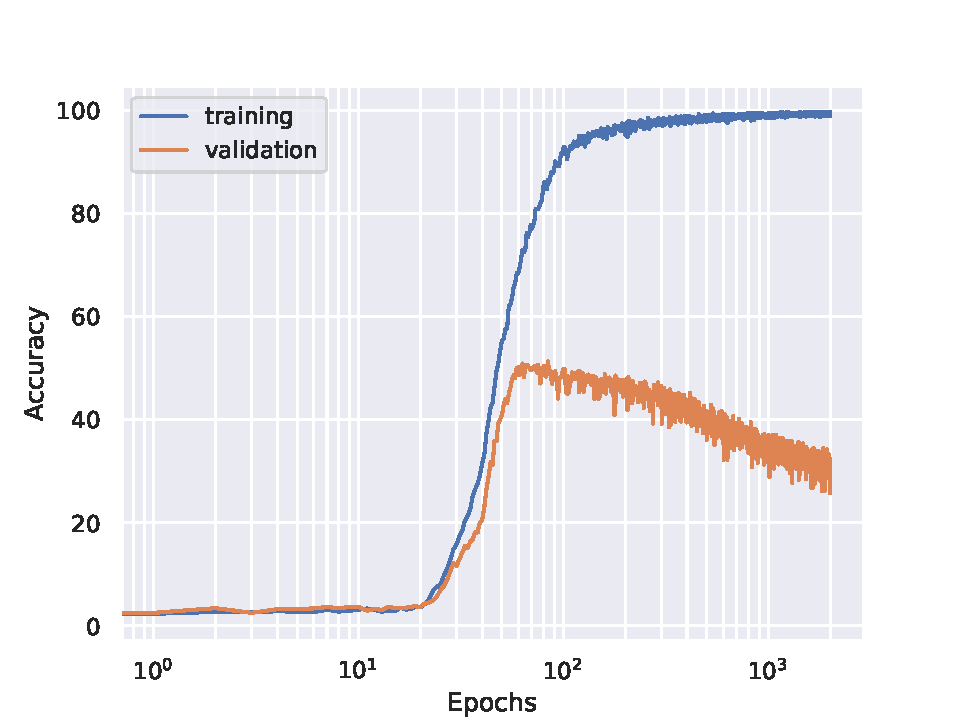
\includegraphics[width=0.35\textwidth]{k4_p97-pre.pdf}\label{k=4}}
  \subfloat[Training and validation accuracy\\ with $K=5$]{
      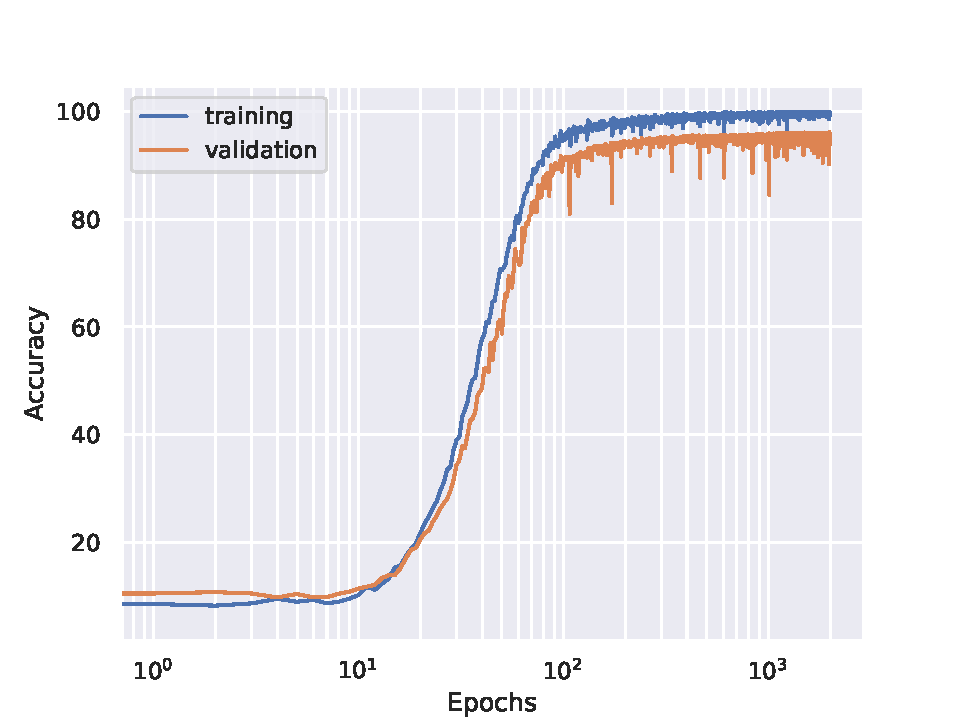
\includegraphics[width=0.35\textwidth]{k5_p97-pre.pdf}\label{k=5}}
  \subfloat[Training and validation accuracy\\ with $K=6$]{
      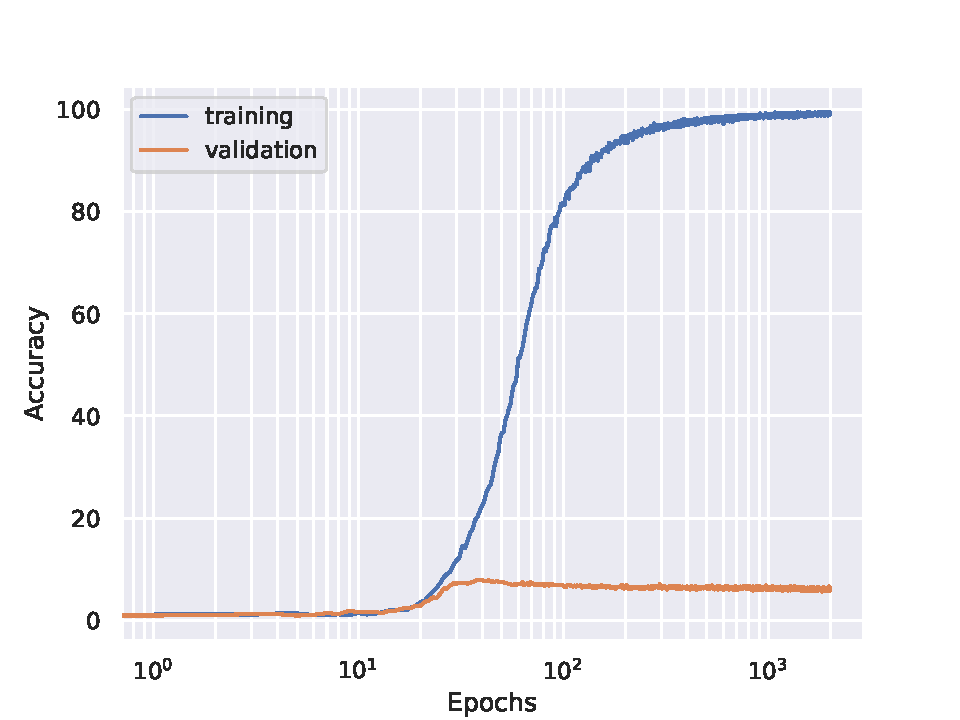
\includegraphics[width=0.35\textwidth]{k6_p97-pre.pdf}\label{k=6}}
  \caption{Grokking phenomenon on transformer model with larger $K$ based on pretrained $K=2$}
  \label{K=4,5,6} 
\end{figure}


\section{Explanation of Grokking}
In this section, we will provide some explanations for the Grokking phenomenon. 
These explanations are mainly based on two aspects: 
the principle of acceleration achieved by the Grokfast algorithm 
and the existing theories that explain the Grokking phenomenon at different stages.


\subsection{Difficulty in learning the low-frequency part of parameters}

According to the experimental results of the Grokfast algorithm, 
the occurrence of the Grokking phenomenon is significantly faster than 
that without using Grokfast. The gap between the reduction of training 
error and the improvement of generalization accuracy has narrowed significantly, 
indicating the success of the Grokfast algorithm in accelerating the 
Grokking phenomenon.


The Grokfast algorithm incorporates an update that amplifies 
the low-frequency components of the gradient after gradient updates, 
while maintaining the rest of the updates unchanged. Therefore, 
its success illustrates an important reason for the Grokking phenomenon: 
the low-frequency components of parameters are difficult to learn. 
During the initial stages of training, the high-frequency components of 
parameters are quickly learned, and these components are sufficient for 
the model to fit the data on the training set, as the amplitude of the 
high-frequency components of parameters is larger, allowing them 
to represent existing data well. However, when generalizing across the 
entire dataset, the high-frequency components of parameters cannot fit 
the low-frequency components of data on the validation set well. 
They can only represent data that is not on the training set very roughly, 
making it difficult to improve generalization accuracy.


In the process of generalization, the model is actually learning the 
low-frequency part of the parameters to more accurately fit the validation set. 
Grokfast enables the model to learn the low-frequency part of the parameters more quickly, 
which makes the generalization of the model faster compared to attain high accuracy 
on the training set. Therefore, an important reason for the Grokking phenomenon is 
the difficulty in learning the low-frequency part of parameters.


\subsection{Existing theoretical explanations at different stages}


According to \cite{lyu2023dichotomy}, the large initialization induces a very strong early phase implicit 
bias towards kernel predictors, but over time, it decays and competes with a late phase 
implicit bias towards min-norm/max-margin predictors induced by the small weight decay, 
resulting in a transition that turns out to be proven sharp in between. 


Briefly, the phenomenon of rapid learning on the training set in the early stages is 
similar to the behavior of kernel predictors, while the phenomenon of gradual 
generalization in the later stages can be explained by min-norm or max-margin predictors 
caused by the small weight decay. The occurrence of the Grokking phenomenon is based 
on the sharp transformation between these two stages, and the characteristics of 
each stage conform to the properties of existing models.Specifically, 
the effectiveness of kernel predictors is closely related to the choice of kernel, 
which can easily lead to overfitting, while min-norm or max-margin predictors have 
stronger robustness and generalization ability. They have a regularization structure, 
thus they learn slower but have less generalization error.
This explanation corresponds precisely to the two stages of the Grokking phenomenon.


In terms of kernel rigime, \cite{mohamadi2024you} provides a more systematic explanation. 
The paper points out that, the dichotomy between early kernel regime and late feature 
learning triggered by weak implicit or explicit regularization seems to be 
the most promising theory to explain grokking. 


The paper also proves that, a wide variety of architectures all fail to generalize 
in the initial phase of training,because networks in the kernel regime can only generalize 
if trained on at least a constant fraction of all possible data points. If this property 
is not satisfied by the training set, then the Grokking phenomenon may not even occur.


In addition, the paper demonstrates that networks with appropriate regularization 
can generalize with many few samples. 
This highlights the importance of regularization in the Grokking phenomenon, 
which plays a crucial role in later generalization.

\appendix

\bibliographystyle{unsrt}
\bibliography{Ref}

\end{document}
